\section{Pronunciation model to WFST}
\label{sec:lexmod}

\subsection{Basic Representation}
\label{subsubsec:lexrep}

From the simple dictionary below, we can construct an L WFST. Figure~\ref{lex} depicts the L WFST.

\begin{Verbatim}[frame=none, framesep=5mm]
<s> sil
</s> sil
bar b ah r
foo f uw
\end{Verbatim}

\begin{figure}[H]
  \centering
  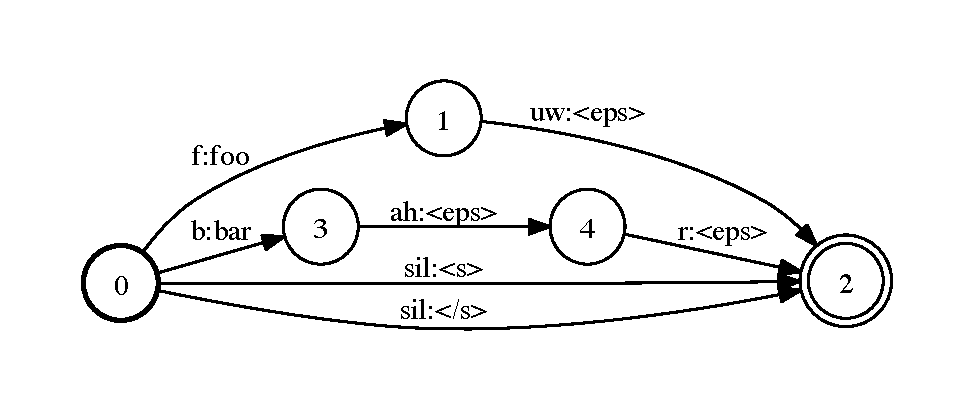
\includegraphics[width=0.6\textwidth]{./figures/lex.pdf}
  \caption{A simple L WFST}
  \label{lex}
\end{figure}

\subsection{Auxiliary Labels}
\label{lexaux}
In general, L is not determinizable in the presence of homophony. To make L determinizable, we need to introduce auxiliary symbols to L. For example\\

\texttt{r eh d \#0} read

\texttt{r eh d \#1} red \\

Let P denotes the maximum degree of the homophony. Then we add P different auxiliary phones.

We need to add a $\phi-$loop at the start state of L. This $\phi-$loop is both to match the $\phi-$labels in G WFST, and to propagate them to the composite WFST of L$^{*}$ and G. 
We also need to add other auxiliary labels (one of \#0, \#1, ... \#P-1) to the end of the phonetic transcription of each word to distinguish homophones. In practice we use the transformed L$^{*}$ to compose.

Figure~\ref{lexstar} depicts the transformed L$^{*}$ WFST.

\begin{figure}[H]
  \centering
  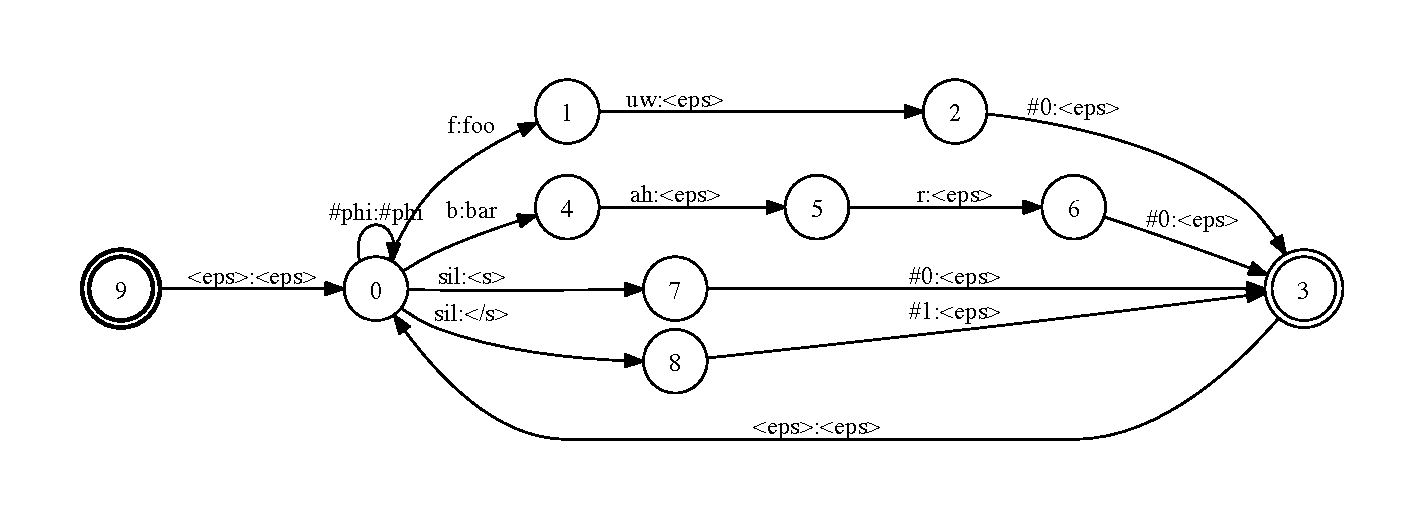
\includegraphics[width=\textwidth]{./figures/lex_star.pdf}
  \caption{A transformed L$^{*}$ WFST}
  \label{lexstar}
\end{figure}

\subsection{Optimization Issues}
\label{lexopt}

We performed experiments on a 4 core Intel Core i3-3220 based machine running at 3.30GHz with 3MB cache and 8GBs of main system memory running GNU/Linux. We evaluated the composing progress using the standard WSJ 5k close NVP bigram language model and the WSJ 5k non-verbalized vocabulary.

To compose L$^{*}$ and G in a standard way, it's preferable not to optimize the L$^{*}$ WFST, since it's optimized to leave the output label in place. Table~\ref{tbl:stdLG} shows the differences of two configurations that optimizes $\tilde{\text{L}}$ or not. The $\circ$ denotes to the standard composition.

\begin{table}[H]
\begin{center}
  \begin{tabular}{| c | c | c | c |}
  \hline
  Composition Configuration & Time & Memory Usage & WFST Size \\ \hline
  $\tilde{\text{L}}\circ\tilde{\text{G}}$ & 0.542s & 47MB & 20MB \\ \hline
  det($\tilde{\text{L}})\circ\tilde{\text{G}}$ & 31.262s & 3.7GB & 891MB \\ \hline
  \end{tabular}
  \caption{Standard composition of $\tilde{\text{L}}$ and $\tilde{\text{G}}$}
  \label{tbl:stdLG}
\end{center}
\end{table}

To compose CL WFST and G WFST with static lookahead approach, C and L$^{*}$ are composed first to produce CL WFST. In this case, it's preferable to determinize L$^{*}$ first. Table~\ref{tbl:lkhCLG} shows the differences of two configurations that optimizes $\tilde{\text{L}}$ or not. The $\circ$ denotes to the standard composition, and the $.$ denotes to the lookahead composition.

\begin{table}[H]
\begin{center}
  \begin{tabular}{| c | c | c | c |}
  \hline
  Composition Configuration & Time & Memory Usage & WFST Size  \\ \hline
  $\tilde{\text{C}}\circ\tilde{\text{L}}$ & 1.601s & 121MB & 68MB \\ \hline
  $(\tilde{\text{C}}\circ\tilde{\text{L}}).\tilde{\text{G}}$ & 4.163s & 315MB & 109MB \\ \hline
  $\tilde{\text{C}}\circ{}det(\tilde{\text{L}})$ & 0.074s & -MB & 1.4MB \\ \hline
  $(\tilde{\text{C}}\circ{}det(\tilde{\text{L}})).\tilde{\text{G}}$ & 3.321s & 183MB & 38MB \\ \hline
  \end{tabular}
  \caption{Static lookahead composition of $\tilde{\text{C}}\tilde{\text{L}}$ and $\tilde{\text{G}}$}
  \label{tbl:lkhCLG}
\end{center}
\end{table}